\documentclass[11pt]{article}

\usepackage[utf8]{inputenc}
\usepackage[T1]{fontenc}
\usepackage{lmodern}
\usepackage[margin=1in]{geometry}
\usepackage{amsmath,amssymb,amsthm,mathtools}
\usepackage{booktabs}
\usepackage{graphicx}
\usepackage{subcaption}
\usepackage{natbib}
\usepackage{hyperref}
\usepackage{xcolor}

\hypersetup{
    colorlinks=true,
    linkcolor=blue!50!black,
    citecolor=blue!50!black,
    urlcolor=blue!50!black
}

\graphicspath{
    {../../outputs/}
    {../../doc/old/figures/cld/}
    {../figures/}
}

\newtheorem{definition}{Definition}
\newtheorem{theorem}{Theorem}
\newtheorem{proposition}{Proposition}
\newtheorem{corollary}{Corollary}
\newtheorem{remark}{Remark}
\newtheorem{assumption}{Assumption}
\newtheorem{example}{Example}
\newtheorem{lemma}{Lemma}

\newcommand{\E}{\mathbb{E}}
\newcommand{\Prob}{\mathbb{P}}
\newcommand{\R}{\mathbb{R}}
\newcommand{\X}{\mathcal{X}}
\newcommand{\Y}{\mathcal{Y}}
\newcommand{\A}{\mathcal{A}}
\newcommand{\metric}{d_{\Y}}
\newcommand{\fstar}{f^\ast}
\newcommand{\concat}{\oplus}
\DeclareMathOperator*{\argmin}{arg\,min}

\title{C-TreePO: Design-Based Partial-Document Supervision for Long-Document Political Measurement}
\author{Mitchell Linegar}
\date{}

\begin{document}
\maketitle

\begin{abstract}
Social scientists increasingly rely on language-model pipelines to turn long documents into measurements, but once texts exceed practical context limits the final coding step is often applied to a compressed representation rather than to the original document itself. Compression is therefore part of the measurement design. This paper introduces \emph{Compression Tree Preference Optimization} (C-TreePO), a design-based framework for long-document political measurement in which the target object is an oracle: the expert or rubric-governed judgment a researcher would trust if full-document evaluation were feasible. Documents are summarized up a compression tree, audited locally for sufficiency, idempotence, and merge consistency, and supervised through random node sampling with logged propensities so compression-induced distortion can be estimated rather than assumed away. The paper links these local checks to oracle-preserving summaries, preference-objective equivalence under explicit oracle-indexing assumptions, and end-to-end design-based certificates for residual gap under partial supervision. We use Manifesto Project RILE scoring as a running illustration and argue more generally that long-document political measurement requires an explicit account of the compression path that produces the object being labeled.
\end{abstract}

\section{Introduction}\label{sec:introduction}

Many core social science problems are, at bottom, problems of disciplined judgment on documents. Researchers want to know which issue positions a party adopts in its manifesto, what priorities a government ranks most highly, whether a speech supports or opposes a policy, or how an expert coder would classify an event described in a long report. In each case the raw text is not the final object of interest. The object of interest is a structured judgment that a researcher or trained expert would produce after reading the full document. That judgment is often expensive, slow, and difficult to scale, which is why the attraction of automated coding remains so strong.

Long documents make this especially difficult. Many political texts are internally structured, context-dependent, and order-sensitive. A manifesto may promise to preserve safe hunting access while also calling for increased mining, fracking, or weaker environmental protections. Those statements do not cancel each other mechanically; their meaning depends on how priorities are ordered, balanced, and qualified across the document. A ranked list of policy priorities, a late-stage caveat, or a tension between two sections can change the final judgment even when the same keywords are present. For these tasks, long-document coding is not just a matter of recovering topics or counting words. It is a matter of preserving the interactions that make a full-document judgment possible.

Older text-as-data approaches are often poorly matched to that problem. Bag-of-words models and topic models offer scalable summaries of document content, but they typically discard order and can flatten precisely the cross-section interactions that matter for substantive interpretation \citep{blei2003latent,roberts2014structural}. Contemporary language models promise something richer. Recent work shows that large language models can recover useful political measurements at scale, including party positions and issue-specific judgments from manifestos and other political texts \citep{BenoitEtAl2025}. But this does not remove the design problem. Once a document is chunked, retrieved, or recursively summarized, the object being scored is no longer the original document. It is a pipeline-produced representation.

That distinction matters because modern language-model pipelines introduce new inferential risks even when headline accuracy looks strong. Design-based Supervised Learning (DSL) shows that substituting imperfect surrogate labels for gold-standard annotations can substantially bias downstream estimates, even when the surrogate appears highly accurate on standard predictive metrics \citep{EgamiEtAl2024}. Long-context models add another failure mode: relevant information in the middle of long inputs is often used unreliably, so longer context windows do not by themselves guarantee faithful full-document judgments \citep{LiuEtAl2024LostMiddle}. In politically contentious domains, further distortions can arise from biases in pretraining corpora and from post-training or alignment procedures designed to shape model behavior \citep{FengEtAl2023PoliticalBias,OuyangEtAl2022InstructGPT,FulayEtAl2024TruthBias}. The problem is therefore not only whether a model predicts the right label on average. It is whether the representation being labeled still preserves the distinctions the researcher cares about.

This paper takes that target object seriously. Formally, I treat the relevant quantity as an \emph{oracle} judgment: the expert, rubric-governed, or otherwise trusted full-information judgment a researcher would want if full-document evaluation were feasible. Many social science coding tasks can be understood this way. Manifesto coding is one example. In the running case of Manifesto Project RILE scoring, the target is not a generic summary of what the manifesto says, but the ideological judgment an expert coding procedure would assign after reading the full manifesto \citep{ManifestoProject2025a}. Preference language is still useful as intuition: the analyst cares about preserving the preference ordering or judgment induced by a trusted evaluator. But the formal object in this paper is narrower and more defensible. It is an oracle-indexed judgment on the full document, not an unrestricted notion of arbitrary human preference.

C-TreePO addresses this problem by treating long-document coding as an oracle-preserving compression problem. A document is partitioned into contiguous spans, summarized into a fixed \emph{Compression Tree}, and audited locally as it is reduced upward. The framework is organized around three locally testable laws. Sufficiency (C1) asks whether a leaf summary preserves the evidence relevant to the oracle. Idempotence (C2) asks whether an already valid summary can be re-summarized without moving the target. Merge Consistency (C3) asks whether combining child summaries preserves the interactions that become visible only when distinct spans are brought together. The claim is intentionally narrow. C-TreePO does not promise generic lossless compression or exact preservation of every downstream use of a text. It asks when local audited summaries preserve an oracle-indexed judgment and how residual distortion can be measured when they do not. In that sense, the framework is closer to task-relative sufficiency in decision theory than to universal semantic fidelity \citep{Blackwell1953}.

The design-based element enters through supervision on the tree itself. Leaves and internal merges form a finite population of audit units. Rather than repeatedly querying the oracle on full documents, the analyst samples nodes for audit, logs inclusion propensities, and uses design-based estimators to quantify compression-induced distortion under a fixed supervision budget. This makes the compression path part of the inferential design rather than a hidden engineering detail. It also connects naturally to preference optimization: when downstream objectives factor through the oracle, local audit information can be used both to certify a compression pipeline and to optimize it. The resulting object is not merely a predicted label, but a labeled compression path accompanied by diagnostics and a design-based account of how much the path can move the target judgment.

The substantive motivation throughout is political measurement, but the technical scope is deliberately bounded. The results apply to oracle-indexed, rubric-governed, or expert-judgment tasks where the relevant distinctions can be expressed on bounded local contexts and audited through the tree. They do not establish correctness for unrestricted preferences or for any downstream objective that distinguishes texts inside the same oracle class. Nor do they guarantee unbiasedness without the transport, calibration, and sampling conditions introduced later in the paper. What the framework offers instead is a transparent route from local audited checks to global claims about distortion, objective gaps, and uncertainty.

The remainder of the paper proceeds in that order. Section~\ref{sec:framework} defines the compression tree and the three local laws. Section~\ref{sec:markov-intuition} introduces the Markov changepoint data-generating process in plain language and shows what information a tree must carry across leaves. Section~\ref{sec:mergeable-intuition} restates the same counting problem in mergeability language, and Section~\ref{sec:semantic-lift} lifts the same mechanism to semantic trees. Section~\ref{sec:po-mapping} connects oracle-preserving compression to preference objectives on summaries, Section~\ref{sec:empirics} reports the main Markov mechanism checks, and Section~\ref{sec:estimation} develops the design-based audit. Section~\ref{sec:scope} clarifies the scope boundary between C-TreePO and the broader Semantic Forests systems agenda, and Section~\ref{sec:conclusion} concludes.

\section{Framework and Local Laws}\label{sec:framework}

\subsection{Setup}

We now fix the main-text setup as explicitly as possible. Let $x\in\X$ be a document, let $g$ be a (possibly stochastic) compression operator, and let $\fstar:\X\to\Y$ be the oracle returning task values of interest. A C-Tree applies $g$ at leaves and then recursively on concatenated child summaries. We compare strings in oracle space with metric $\metric$.

\begin{assumption}[Fixed C-Tree Structure]\label{ass:fixed-structure}
For each document $x$, the C-Tree topology and leaf partition are treated as fixed throughout optimization and auditing in the main text.
\end{assumption}

Assumption~\ref{ass:fixed-structure} is a notational simplification, not a restriction of principle. It isolates representation quality from partition randomness so the local-to-global argument can be read directly. Appendix~\ref{app:fixed-partition} then shows the same preservation logic holds for any deterministic partition rule that maps each document to a fixed realized tree.

\begin{definition}[Oracle Equivalence]
For strings/spans $u,v$, define $u\sim v$ iff $\metric(\fstar(u),\fstar(v))=0$.
\end{definition}

\begin{assumption}[Context Compatibility]\label{ass:context-compat}
For all strings $u,v,w$, if $u\sim v$ then both $w\concat u\sim w\concat v$ and $u\concat w\sim v\concat w$.
\end{assumption}

Keep one toy document in view throughout. It will reappear in Section~\ref{sec:markov-intuition}. For any span, write its state as
\[
(c,a,b)= (\text{changepoints inside the span},\ \text{first color},\ \text{last color}).
\]
In the one-leaf baseline, the whole document is one span, so there is no merge problem yet. For the toy document
\[
\text{Blue Blue Blue}\ \mid\ \text{Orange Orange Green}\ \mid\ \text{Green Red Red}\ \mid\ \text{Blue Blue Orange},
\]
the full-span state is $(5,\text{Blue},\text{Orange})$: there are five color changes, the span starts in Blue, and it ends in Orange. This is the easy case. Nothing has to be reconstructed across leaves because there are no leaves yet.

The real problem appears only after the fixed partition turns that same document into four leaves:
\[
\mathrm{L}_1=(0,\text{Blue},\text{Blue}),\quad
\mathrm{L}_2=(1,\text{Orange},\text{Green}),\quad
\mathrm{L}_3=(1,\text{Green},\text{Red}),\quad
\mathrm{L}_4=(1,\text{Blue},\text{Orange}).
\]
Now the problem becomes real. Each leaf summary has to preserve not only how many changes happened inside the leaf, but also the colors at the leaf's left and right edges. Those edge colors are what later merges need. In this toy setting the parent and root states are recovered by the join rule
\[
(c_L,a_L,b_L)\otimes(c_R,a_R,b_R)
=
\big(c_L+c_R+\mathbf{1}\{b_L\neq a_R\},\ a_L,\ b_R\big),
\]
so preserving a span means preserving the whole triple $(c,a,b)$, not just a leaf-local count.

This is also the first concrete example of the kind of oracle-indexed preference the paper studies. Here the preference is extremely simple: the good summaries are the ones that let the tree keep the final changepoint count correct. The learner does not need a theory of what ``Blue'' means. It only needs to discover which compressed leaf states make the root answer come out right. That immediately favors summaries that carry boundary information rather than summaries that only look adequate inside one leaf.

The C-Tree audit uses three local laws. Each is checked on a small local prompt, but together they control the final tree output:
\begin{align*}
\text{(C1) Sufficiency:}\quad & g(b)\sim b\quad\text{for every realized leaf }b,\\
\text{(C2) Idempotence:}\quad & g(s)\sim s\quad\text{for every }s\in\operatorname{range}(g),\\
\text{(C3) Merge Consistency:}\quad &
u\concat v\sim g(u\concat v)\sim g\big(g(u)\concat g(v)\big)\quad\text{for all }u,v.
\end{align*}

Each law corresponds to one simple failure mode. C1 says a leaf summary must preserve what matters. C2 says an already-good summary should not drift when it is compressed again. C3 says merging two good child summaries should still give the right parent state.

\begin{figure}[t]
    \centering
    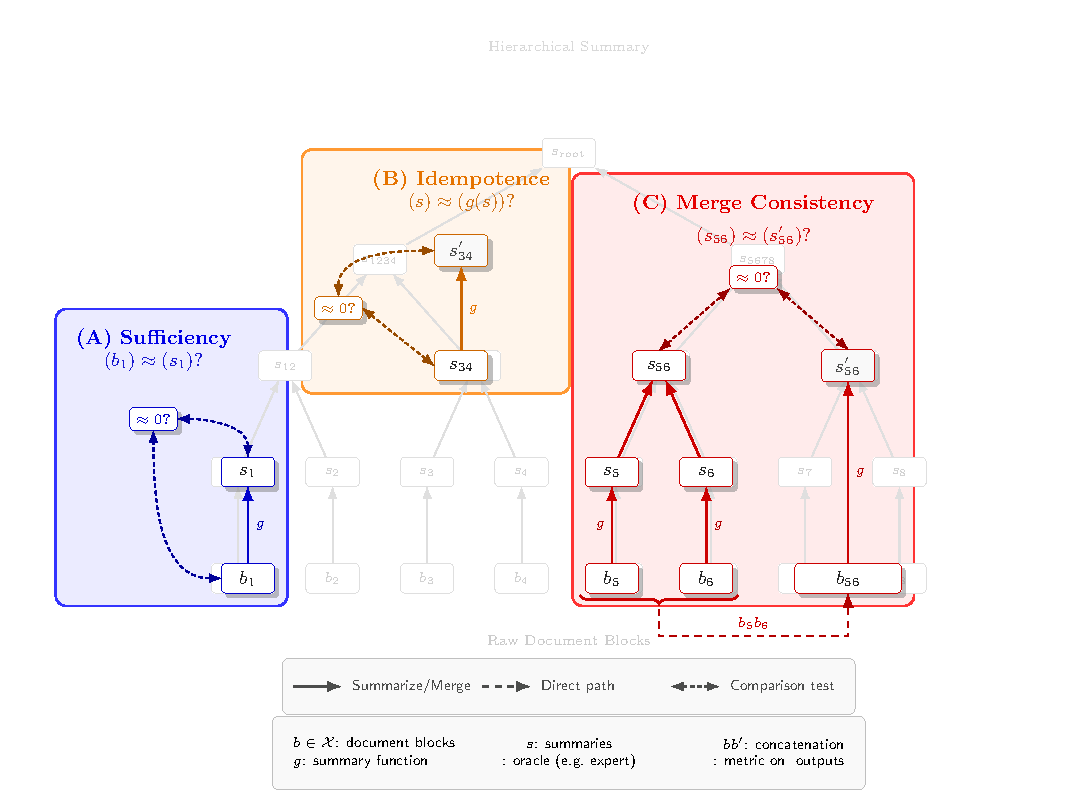
\includegraphics[width=0.95\linewidth]{05_full.pdf}
    \caption{Spotlight view of the three local laws on a realized tree.
    Gray nodes are context; colored panels are the auditable local prompts.
    Read each highlighted panel as checking whether a span state $(c,a,b)$ survives the corresponding local operation.}
    \label{fig:local-laws-full}
\end{figure}

Figure~\ref{fig:local-laws-full} is easiest to read through this color example. Panel (A) is C1. If a leaf contains Orange Orange Green, then the summary has to preserve $(1,\text{Orange},\text{Green})$. If it forgets either boundary color, a later merge can miss a cross-leaf changepoint. Panel (B) is C2. Once a summary already encodes the right state for a span, compressing it again should not change that state. Otherwise the tree can change its answer even though no new evidence was added.

Panel (C) is C3. This is the rule that makes the tree compositional. In the running example,
\[
\mathrm{L}_1=(0,\text{Blue},\text{Blue})
\quad\text{and}\quad
\mathrm{L}_2=(1,\text{Orange},\text{Green})
\]
must merge to
\[
\mathrm{P}_{12}=(2,\text{Blue},\text{Green}),
\]
because the parent count is $0+1+1=2$: one change inside $\mathrm{L}_2$ and one extra change at the boundary Blue $\rightarrow$ Orange. The same rule gives
\[
\mathrm{P}_{34}=(3,\text{Green},\text{Orange})
\quad\text{and}\quad
\mathrm{Root}=(5,\text{Blue},\text{Orange}),
\]
which is the full-document state we started from in the one-leaf baseline. That same state is drawn explicitly later in Figure~\ref{fig:markov-tree-state}.

\subsection{Proof Strategy}

The paper's proofs are intentionally constructive. Each global claim is decomposed into local invariance steps involving tree structure, oracle measurability, and design-based estimation, then recomposed by induction or triangle inequality. To make this auditable, Appendix~\ref{app:proof-map} provides a map from each result to its full proof location, and each appendix proof cites the corresponding Lean theorem anchors.

\section{A Simple Tree Intuition: Markov Changepoints}\label{sec:markov-intuition}

\subsection{The Data-Generating Process}

The main-text simulations use a deliberately simple task. Each document has 128 observed tokens. Behind those tokens is a hidden color sequence that stays the same for a while and then switches. Each hidden color generates words from its own small vocabulary. In the toy example, this is made completely literal: Blue states emit blue words, Orange states emit orange words, and so on. The document-level label is just the total number of color changes across the full sequence.

That is simple enough to describe exactly, but it still captures the main long-document problem. The learner never sees the hidden colors, the true boundaries, or the changepoints. It only sees the words and the supervision provided during training. In the root-only experiments below, the neural operator gets document-level labels only. It is not told which tokens belong to which hidden color or where the local switches happened. Just as importantly, it is not asked to recover the full hidden path. Its only job is to estimate the total number of changes in the document. The 12-token toy document used here is the same one already used to explain the local laws:
\[
\text{Blue Blue Blue}\ \mid\ \text{Orange Orange Green}\ \mid\ \text{Green Red Red}\ \mid\ \text{Blue Blue Orange}.
\]
Its full-span state is $(5,\text{Blue},\text{Orange})$.

This is why the example is useful. The supervision is global and task-specific. The model is not rewarded for reconstructing the whole hidden path or for explaining the sequence token by token. It is rewarded only for getting the document-level judgment right. In that sense, the Markov task is already a tiny preference-learning problem: the objective prefers the outputs that preserve the correct final count.

\begin{figure}[t]
    \centering
    \includegraphics[width=\linewidth]{markov_changepoint_dgp_slide.pdf}
    \caption{Plain-language view of the Markov changepoint simulation for the same toy document used in the local-law discussion. The hidden color path generates the observed words, but the learner does not observe that path directly. The target is the number of regime changes in the full document, and the leaf partition is fixed before training.}
    \label{fig:markov-dgp}
\end{figure}

Figure~\ref{fig:markov-dgp} shows the data-generating process on that toy document. The hidden path is shown only for explanation. In the real learning problem, the model has to infer from the words alone which boundaries matter for the final count.

\subsection{Why Tree Reduction Is Hard}

If the whole document is processed as one span, the task is conceptually direct: count how many times the hidden color changes from left to right. Tree reduction makes the task harder because the relevant evidence is often split across leaf boundaries. A leaf can look simple internally while still ending in a different color from the one that begins the next leaf.

This is why leaf size matters. As leaves get shorter, the document is broken into more spans and the tree has to reason about more boundaries. The exact leaves-per-document used in the plotted runs appear on the horizontal axis of Figures~\ref{fig:markov-recoverable-leaf-size} and \ref{fig:markov-structural-leaf-size}. The important point is simple: smaller leaves create more places where a changepoint can disappear if the summary forgets boundary state.

That same structure also explains why this setting favors learning across boundaries. Root supervision cannot reward a leaf summary just for looking plausible on its own. A summary is useful only if it helps the parent decide whether the next span contributes one more changepoint. Two leaves can have the same internal count and still lead to different root answers depending on how their boundary colors line up. So the training signal pushes the learner toward summaries whose value appears at merge time.

\begin{figure}[t]
    \centering
    \includegraphics[width=\linewidth]{markov_changepoint_combined_slide_v2.pdf}
    \caption{The same toy document reduced through a four-leaf tree. Each node stores the span state $(c,a,b)$, where $c$ is the number of changepoints inside the span, $a$ is the first color, and $b$ is the last color. The parent states are forced by the merge rule already used to explain C1--C3.}
    \label{fig:markov-tree-state}
\end{figure}

\subsection{What the Tree Must Learn}

Figure~\ref{fig:markov-tree-state} is the concrete version of the state tuple introduced above. A good leaf summary has to preserve two things at once: what happened inside the leaf, and how the leaf begins and ends. In this notation, $c$ counts the changes already inside the span, $a$ stores the left boundary color, and $b$ stores the right boundary color. Without those boundary colors, a parent node cannot tell whether two neighboring summaries should add one more cross-leaf changepoint when they are merged.

This is the central C-Tree intuition in its cleanest form. The important information is not always inside one leaf. Sometimes it lives in the relation between neighboring leaves. In the Markov task, the learner has to discover from root-level supervision which compressed leaf states are useful for recovering those cross-leaf interactions. If the summary forgets what happens at the edges, the root cannot systematically recover the right answer. The next section states the same idea in the language of mergeable summaries.

\section{A Short Mergeability Analogy}\label{sec:mergeable-intuition}

The Markov example already contains the whole mechanism. In this toy setting we are not trying to recover a rich latent structure or classify each token separately. We are trying to estimate one number: the total number of changes in the full document. So the compression question is narrow and concrete. What must each leaf pass upward so that the tree can keep counting correctly after the document has been split?

\subsection{Count the Changes}

\begin{definition}[Change-count Sufficiency]
In the Markov toy task, a span summary is change-count sufficient if it preserves three objects for that span: the number of internal regime changes, the first regime, and the last regime.
\end{definition}

\begin{proposition}[Failure Boundary for Count-Only Summaries]\label{prop:m_lt_k}
If a leaf summary retains only the number of changes inside each leaf and discards boundary state, then there exist partitioned documents with identical retained leaf summaries but different full-document change counts. Hence count-only summaries are information-limited for the toy task.
\end{proposition}

The intuition is immediate. Consider two two-leaf documents:
\[
\text{Blue Blue Blue}\ \mid\ \text{Orange Orange Orange},
\qquad
\text{Blue Blue Blue}\ \mid\ \text{Blue Blue Blue}.
\]
In both cases the leaf-internal counts are $(0,0)$: neither leaf contains a regime change inside itself. But the full-document answers differ. The first document has one change at the leaf boundary Blue $\rightarrow$ Orange; the second has zero. If the tree propagates only leaf-internal counts, the root sees the same retained state for both documents and cannot recover the correct total. The ambiguity is structural and remains even with infinite data.

This is the whole toy mechanism. The root is trying to estimate the total number of changes, and every merge has the form
\[
 c_{\mathrm{parent}} = c_L + c_R + \mathbf{1}\{b_L \neq a_R\}.
\]
The first two terms count changes already known to live inside the left and right child spans. The last term asks whether crossing the boundary between those spans contributes one additional change. That boundary term is why a merge-safe summary must preserve more than a local count. In the Markov task, the extra information is exactly the boundary state. The analogy to mergeable sketches is therefore simple: a good summary is not whatever is compact, but whatever still lets the tree keep counting changes after repeated merges.

\section{From Counting Changes to Semantic C-Trees}\label{sec:semantic-lift}

The toy task is simple: detect when the color changes. A leaf-local count fails because the root also needs to know whether one extra change appears at the boundary between two leaves. The semantic case has the same shape. Replace colors with claims, qualifications, references, or priorities. A summary can look adequate inside one span and still fail because it hides the relation between neighboring spans.

What changes between the numeric and semantic settings is the form of the summary, not the logic. In the Markov example, the useful summary is the tuple $(c,a,b)$. In a semantic task, the useful summary may be a short textual state. But the tree is doing the same job in both cases: carry forward enough information so later merges can reconstruct the full-document judgment the oracle prefers. C1 says preserve what matters at the leaf. C2 says do not corrupt it when the summary is compressed again. C3 says the merge step must preserve what matters on the combined span. The Markov example is therefore not a side case. It is the simplest running example of an oracle-indexed preference that is easy to state, globally supervised, and driven by cross-boundary information.

\begin{definition}[Additively Separable and Not Additively Separable Tree Utilities]\label{def:nonseparable}
A tree-level utility $U$ is additively separable if there exist leaf-local functions $\{h_u\}$ such that
\[
U(T)=\sum_{u\in\mathrm{Leaves}(T)} h_u(s_u)
\]
for all realized trees in the support. A utility is not additively separable when the correct answer also depends on relations across leaves.
\end{definition}

\begin{example}[Explicit Not Additively Separable Changepoint Utility]\label{ex:changepoint-nonseparable}
Let two child spans carry states
\[
s_L=(c_L,a_L,b_L),\qquad s_R=(c_R,a_R,b_R),
\]
and define the parent utility
\[
U(s_L,s_R)=c_L+c_R+\mathbf{1}\{b_L\neq a_R\}.
\]
This utility is not additively separable over leaf-local pieces because the boundary term cannot be assigned to either child alone. Proposition~\ref{prop:m_lt_k} gives the simplest failure case: two partitioned documents can have the same retained leaf counts and still require different root answers because the cross-leaf boundary differs. The semantic version is the same whenever one span changes how the next span should be read, for example when a later sentence qualifies, negates, or reorders what came before.
\end{example}

This is the point of the semantic lift. It is not enough to score each leaf independently and add the scores. The tree must preserve the cross-span information the oracle uses. In the Markov task, that information is just the boundary color. In semantic tasks, it may be a boundary condition, a cross-reference, a temporal qualifier, a contradiction, or an ordering relation. The content changes, but the logic does not.

\section{C-TreePO as Preference Optimization}\label{sec:po-mapping}

\subsection{Data-generating object}

For document $x$, Assumption~\ref{ass:fixed-structure} gives a fixed realized tree structure, and policy $\pi_\theta$ induces randomness only through node-level generation, compression, and scoring decisions on that structure. We write the resulting random C-Tree as $T\sim\pi_\theta(\cdot\mid x)$:
\[
T = \mathrm{BuildTree}(x,\mathcal{T}(x);\theta,\xi),
\]
where $\xi$ denotes internal stochasticity. Preference supervision is collected over paired trees $(T^+,T^-)$.

The same formal mapping extends to any deterministic partition rule $\Pi$ with $x\mapsto\mathcal{T}_\Pi(x)$, because conditioning on $\mathcal{T}_\Pi(x)$ returns the identical fixed-structure argument. Appendix~\ref{app:fixed-partition} gives the explicit statement and proof.

\subsection{Objective layer}

For pairwise optimization (DPO style), the tree-level objective is:
\[
\mathcal{L}_{\mathrm{DPO}}(\theta)
= -\E\!\left[\log\sigma\!\left(
\beta\log\frac{\pi_\theta(T^+\mid x)}{\pi_{\mathrm{ref}}(T^+\mid x)}
-\beta\log\frac{\pi_\theta(T^-\mid x)}{\pi_{\mathrm{ref}}(T^-\mid x)}
\right)\right].
\]
Listwise and RL-style objectives use tree groups and tree-indexed rank/reward definitions analogously.

\subsection{Core guarantees}

\begin{theorem}[Preservation Under Local Laws]\label{thm:preservation}
Assume C1--C3 hold on realized C-Tree leaves and internal edges.
Then the expected oracle distortion between the C-Tree output and the original document is zero:
\[
\E\left[\metric\big(\fstar(Z^{(R)}(x)),\fstar(x)\big)\right]=0\quad\text{for }R\ge1.
\]
\end{theorem}

The proof is inductive over tree structure and rounds. C1 handles leaves, C3 transports equivalence across merges, and C2 controls re-summarization rounds. The corresponding Lean theorem is \texttt{multi\_round\_proper}.

\begin{theorem}[Preference-Objective Equivalence]\label{thm:equiv}
Under oracle-measurability/indexing conditions for policies, generators, and rewards/rankers,
training objectives on C-Tree summaries equal corresponding objectives on originals.
For nonzero distortion $\Delta_R$, objective differences satisfy method-specific Lipschitz bounds:
\[
\left|\E[\mathcal{L}(X)]-\E[\mathcal{L}(Z)]\right| \le L\,\Delta_R.
\]
\end{theorem}

Lean anchors for Theorem~\ref{thm:equiv} are \texttt{dpo\_equivalence}, \texttt{grpo\_equivalence}, \texttt{grpo\_rl\_equivalence}, and \texttt{unified\_preference\_gap\_bounded}.

\begin{theorem}[End-to-End C-TreePO Certificate]\label{thm:e2e}
With logged propensities and design-based sampling,
Horvitz--Thompson style estimators of C-Tree objective terms are unbiased (or controlled in clipped/noisy variants),
and method-level DPO/GRPO gap certificates follow by composition.
\end{theorem}

\subsection{Map of Full Proofs}

Table~\ref{tab:proof-map-main} shows where each complete proof appears in the appendix.
The detailed theorem-to-Lean crosswalk is moved to Appendix~\ref{app:lean-crosswalk}.
A supporting extension theorem covering arbitrary deterministic fixed partition rules appears in Appendix~\ref{app:fixed-partition}.

\begin{table}[t]
\centering
\small
\begin{tabular}{p{0.42\linewidth}p{0.45\linewidth}}
\toprule
Result in Main Text & Full proof location \\
\midrule
Proposition~\ref{prop:m_lt_k} (count-only failure boundary) & Appendix~\ref{app:proof-m-lt-k} \\
Theorem~\ref{thm:preservation} (local laws $\Rightarrow$ preservation) & Appendix~\ref{app:proof-preservation} \\
Theorem~\ref{thm:equiv} (preference-objective equivalence and gap bound) & Appendix~\ref{app:proof-equivalence} \\
Theorem~\ref{thm:e2e} (end-to-end certificate) & Appendix~\ref{app:proof-e2e} \\
\bottomrule
\end{tabular}
\caption{Map of where each full proof is written out in detail.}
\label{tab:proof-map-main}
\end{table}

C-TreePO is best described as a compression-tree data and estimation framework that enables standard preference optimizers with explicit distortion and estimation certificates.

\section{Markov Empirical Patterns}\label{sec:empirics}

The main-text evidence now focuses only on the Markov changepoint family introduced above. Throughout these figures, the learner sees observed tokens and root labels only. It does not observe the hidden regime path, the local changepoints inside leaves, or any explicit token-to-regime mapping. The question is whether a tree trained from that limited supervision can still learn summaries that preserve the global count of regime changes as leaf geometry becomes more demanding.

\begin{figure}[t]
    \centering
    \includegraphics[width=\linewidth]{markov_v3_publication_leaf_size_fixed_docs_20260414_040020/figures/recoverable_root_only_leaf_size_fixed_train10240.png}
    \caption{Recoverable Markov case at a fixed training-set size of 10,240 documents. Documents have 128 tokens, 4 hidden regimes, and 2--6 contiguous segments. Panels vary the share of training documents that receive root labels. The substantive comparison is the root-only tree curve against the full-document FNO reference at leaf128. In this simple case, making leaves smaller mostly hurts because it creates more boundaries the tree must reconstruct from root supervision alone.}
    \label{fig:markov-recoverable-leaf-size}
\end{figure}

Figure~\ref{fig:markov-recoverable-leaf-size} is the simple recoverable case. When the document is kept as one leaf, the task is nearly trivial because the model can process the whole sequence directly. Once the same document must be represented as multiple leaves, error rises because the tree has to infer cross-leaf boundary structure from document-level labels alone. The deterioration is modest when root supervision is abundant and much sharper when root labels are scarce.

\begin{figure}[t]
    \centering
    \includegraphics[width=\linewidth]{markov_v3_publication_leaf_size_fixed_docs_20260414_040020/figures/structural_root_only_leaf_size_fixed_train10240.png}
    \caption{Harder Markov case at the same fixed training-set size of 10,240 documents. Documents still have 128 tokens, but now the latent process uses 12 hidden regimes and 10--12 contiguous segments. The one-leaf full-document FNO baseline is much weaker here, while the tree improves sharply once it can use multiple leaves and learned merges. The best operating point is no longer the one-leaf model; it is a multileaf tree that preserves enough boundary information without making the merge problem too deep.}
    \label{fig:markov-structural-leaf-size}
\end{figure}

Figure~\ref{fig:markov-structural-leaf-size} shows the harder structural version of the same problem. Here the document must represent many more latent identities and many more boundary events within the same 128-token budget. That change flips the comparative picture. A one-leaf full-document baseline is no longer strong, because the flat model has to solve the entire counting problem in one pass. A tree with moderate leaf granularity does better because it can learn local summaries and then aggregate them upward. But the gain is not free: when leaves become too small, the model again pays a penalty because the merge burden becomes too large.

\section{Estimation, Auditing, and Honesty}\label{sec:estimation}

C-TreePO relies on sampled oracle queries.
For queried unit $i$ with inclusion indicator $Z_i$, propensity $\pi_i$, and contribution $R_i$, the HT estimator is:
\[
\hat{J}_{\mathrm{HT}} = \frac{1}{n}\sum_i \frac{Z_i}{\pi_i}R_i.
\]

Adaptive chunking and learned judges introduce interference paths.
To keep evaluation valid, reporting must be honest with respect to adaptation roles (chunker, summarizer, oracle): adaptation on train-role partitions, evaluation on held-out role intersections.
The same discipline applies to simulation sweeps with tunable local-law weights: hyperparameter selection belongs on a validation split, and the paper's quantitative claims should be reported on a disjoint test split. Any plots that optimize on the same held-out slice they report are exploratory diagnostics rather than confirmatory evidence.

A practical bound stack decomposes target error into calibration, estimation, and clipping envelopes.
For true gap $G^\ast$, judge-view $G^J$, sampled estimate $G^E$, and clipped estimate $G^C$:
\[
|G^\ast-G^C| \le |G^\ast-G^J| + |G^J-G^E| + |G^E-G^C|.
\]
Event-based concentration and union composition then yield one-shot high-probability certificates.

\section{Scope and Relation to Semantic Forests}\label{sec:scope}

C-TreePO is intended for long-context settings in which full-document oracle usage is too expensive, local bounded checks are feasible, and utility-relevant information can be propagated through compression states.

Likely failure modes include irreducibly nonlocal tasks, severe support collapse, and unstable calibration transfer.

This paper should own the method and certificate core (local laws, objective mapping, estimation guarantees).
The Semantic Forests paper should own system-scale orchestration, deployment engineering, and broad cross-domain throughput/robustness analysis.

\section{Conclusion}\label{sec:conclusion}

C-TreePO provides a concrete local-to-global route for long-document preference optimization.
The draft's argument is intentionally staged: Markov data-generating process first, boundary-state intuition next, a short counting-based mergeability discussion after that, and then formal semantic preference and estimation mapping.
The resulting picture is pragmatic: local checks become optimization signals, design-based estimators control uncertainty, and global preference claims are made through explicit certificates rather than implicit trust in truncation.

\appendix

\section{Proof Map and Lean Crosswalk}\label{app:proof-map}

\subsection{Proof Map}

\begin{table}[h]
\centering
\small
\begin{tabular}{p{0.34\linewidth}p{0.24\linewidth}p{0.36\linewidth}}
\toprule
Result & Appendix proof section & Lean reference section \\
\midrule
Theorem~\ref{thm:fixed-partition} & Appendix~\ref{app:fixed-partition} & Appendix~\ref{app:lean-crosswalk} \\
Proposition~\ref{prop:m_lt_k} & Appendix~\ref{app:proof-m-lt-k} & Appendix~\ref{app:lean-crosswalk} \\
Theorem~\ref{thm:preservation} & Appendix~\ref{app:proof-preservation} & Appendix~\ref{app:lean-crosswalk} \\
Theorem~\ref{thm:equiv} & Appendix~\ref{app:proof-equivalence} & Appendix~\ref{app:lean-crosswalk} \\
Theorem~\ref{thm:e2e} & Appendix~\ref{app:proof-e2e} & Appendix~\ref{app:lean-crosswalk} \\
\bottomrule
\end{tabular}
\caption{Navigation map for all full proofs in this draft.}
\end{table}

\subsection{Lean Crosswalk}\label{app:lean-crosswalk}

\begin{table}[h]
\centering
\small
\begin{tabular}{p{0.34\linewidth}p{0.30\linewidth}p{0.30\linewidth}}
\toprule
Paper result & Lean theorem name(s) & Lean file \\
\midrule
Theorem~\ref{thm:fixed-partition} &
\texttt{multi\_round\_proper} (instantiated for arbitrary fixed tree) &
\texttt{lean3/FormalProofs/OPT/ExpectationTheory.lean} \\

Theorem~\ref{thm:preservation} &
\texttt{multi\_round\_proper} &
\texttt{lean3/FormalProofs/OPT/ExpectationTheory.lean} \\

Theorem~\ref{thm:equiv} (exact case) &
\texttt{dpo\_equivalence}, \texttt{grpo\_equivalence}, \texttt{grpo\_rl\_equivalence} &
\texttt{lean3/FormalProofs/OPT/PreferenceLearning.lean} \\

Theorem~\ref{thm:equiv} (gap bound) &
\texttt{unified\_preference\_gap\_bounded} &
\texttt{lean3/FormalProofs/OPT/PreferenceBounds.lean} \\

Theorem~\ref{thm:e2e} (objective unbiasedness) &
\texttt{treepo\_objective\_unbiased}, \texttt{treepo\_distortion\_unbiased} &
\texttt{lean3/FormalProofs/DSL/TreePOEndToEnd.lean} \\

Theorem~\ref{thm:e2e} (method certificates) &
\texttt{dpo\_treepo\_end\_to\_end\_certificate}, \texttt{grpo\_pl\_treepo\_end\_to\_end\_certificate}, \texttt{grpo\_rl\_treepo\_end\_to\_end\_certificate} &
\texttt{lean3/FormalProofs/DSL/TreePOEndToEnd.lean} \\

Sketch-transport component used in Theorem~\ref{thm:e2e} discussion &
\texttt{dpo\_tree\_gap\_bounded\_by\_sketch\_upper}, \texttt{grpo\_pl\_tree\_gap\_bounded\_by\_sketch\_upper}, \texttt{grpo\_rl\_tree\_gap\_bounded\_by\_sketch\_upper} &
\texttt{lean3/FormalProofs/DSL/MergeableCertificates.lean} \\
\bottomrule
\end{tabular}
\caption{Theorem-to-Lean crosswalk (moved to appendix).}
\end{table}

\section{Fixed-Partition Extension}\label{app:fixed-partition}

\begin{theorem}[Extension to Any Deterministic Fixed Partition]\label{thm:fixed-partition}
Let $\Pi$ be any deterministic rule that maps each document $x$ to a finite ordered rooted tree $\mathcal{T}_\Pi(x)$ with contiguous leaves. For each $x$, construct C-Tree summaries on $\mathcal{T}_\Pi(x)$ and assume C1--C3 hold almost surely on all realized leaf and merge calls. Then for every round $R\ge 1$,
\[
\E\!\left[\metric\!\big(\fstar(Z_\Pi^{(R)}(x)),\fstar(x)\big)\,\middle|\,x\right]=0.
\]
Consequently, for any distribution over documents $X$,
\[
\E\!\left[\metric\!\big(\fstar(Z_\Pi^{(R)}(X)),\fstar(X)\big)\right]=0.
\]
\end{theorem}

\begin{proof}
Fix $x$ and condition on the realized tree $\mathcal{T}_\Pi(x)$. Because $\Pi$ is deterministic, the tree is fixed under this conditioning, so Theorem~\ref{thm:preservation} applies directly and yields
\[
\E\!\left[\metric\!\big(\fstar(Z_\Pi^{(R)}(x)),\fstar(x)\big)\,\middle|\,x,\mathcal{T}_\Pi(x)\right]=0.
\]
Since $\mathcal{T}_\Pi(x)$ is a measurable function of $x$, the same equality holds conditioning only on $x$. Taking expectation over $X$ and applying the tower property gives the unconditional statement.
\end{proof}

Lean correspondence for Theorem~\ref{thm:fixed-partition} follows from the same formal theorem used in Theorem~\ref{thm:preservation}, namely \texttt{multi\_round\_proper} in \texttt{lean3/FormalProofs/OPT/ExpectationTheory.lean}, instantiated at an arbitrary fixed tree.

\section{Full Proof of Proposition~\ref{prop:m_lt_k}}\label{app:proof-m-lt-k}

\begin{proof}
Fix a deterministic two-leaf partition and suppose each leaf summary retains only the number of regime changes inside that leaf.
Equivalently, the summary map discards the left and right boundary regimes and outputs only an internal count.

Construct two partitioned documents with the same leaf geometry:
\[
x^- = \text{Blue Blue Blue}\ \mid\ \text{Orange Orange Orange},
\qquad
x^+ = \text{Blue Blue Blue}\ \mid\ \text{Blue Blue Blue}.
\]
Let $S(\cdot)$ denote the retained pair of leaf-internal counts.
For both documents, neither leaf changes regime inside the leaf, so
\[
S(x^-)= (0,0)=S(x^+).
\]
However, the full-document changepoint counts differ.
In $x^-$ there is one regime change at the leaf boundary Blue $\rightarrow$ Orange, whereas in $x^+$ there is no boundary change.
Hence
\[
f^\star(x^-)=1,\qquad f^\star(x^+)=0.
\]
Therefore two inputs with identical retained leaf summaries yield different full-document targets.
No estimator restricted to count-only summaries can recover the toy changepoint target without ambiguity.
This proves that discarding boundary state creates an information-limited failure.
\end{proof}

The exact impossibility lemma above is currently not exposed as a standalone theorem name in the Lean tree.
The closest formal bridge for this paper's certificate path is in
\texttt{lean3/FormalProofs/DSL/MergeableCertificates.lean} and
\texttt{lean3/FormalProofs/OPT/MergeableReduction.lean}.

\section{Full Proof of Theorem~\ref{thm:preservation}}\label{app:proof-preservation}

\begin{proof}
Fix a realized full binary C-Tree $T$ over document $x$.
For each node $u$, define latent raw span $S(u)$ recursively by setting $S(u)=b$ when $u$ is a leaf containing block $b$, and setting $S(u)=S(u_L)\concat S(u_R)$ when $u$ is an internal node with children $(u_L,u_R)$.
Define stored summary $s_u$ recursively by setting $s_u=g(S(u))$ at leaves and $s_u=g(s_{u_L}\concat s_{u_R})$ at internal nodes.
Let $r$ be the root and set $Z^{(1)}(x):=s_r$.
Assume C1--C3 hold almost surely on all realized calls.

We first show $s_u\sim S(u)$ for every node $u$ by structural induction on node height. If $u$ is a leaf, C1 gives $s_u=g(S(u))\sim S(u)$. For the inductive step, assume $s_{u_L}\sim S(u_L)$ and $s_{u_R}\sim S(u_R)$.
By context compatibility,
\[
s_{u_L}\concat s_{u_R}\sim S(u_L)\concat S(u_R)=S(u).
\]
By C3 (applied to $u=s_{u_L}$ and $v=s_{u_R}$),
\[
g(s_{u_L}\concat s_{u_R})\sim s_{u_L}\concat s_{u_R}.
\]
Since $s_u=g(s_{u_L}\concat s_{u_R})$, transitivity gives $s_u\sim S(u)$.
This completes induction.

At root $r$, we have $s_r\sim S(r)=x$, hence
\[
\metric\!\big(\fstar(Z^{(1)}(x)),\fstar(x)\big)=0
\]
almost surely, so
\[
\E\!\left[\metric\!\big(\fstar(Z^{(1)}(x)),\fstar(x)\big)\right]=0.
\]

Define rounds by $Z^{(R+1)}(x):=g(Z^{(R)}(x))$ for $R\ge1$.
Because $Z^{(1)}(x)=s_r\in\operatorname{range}(g)$ and $g$ maps into its range, each $Z^{(R)}(x)$ is in $\operatorname{range}(g)$.
By C2:
\[
Z^{(R+1)}(x)\sim Z^{(R)}(x)\quad\text{for all }R\ge1.
\]
We prove $Z^{(R)}(x)\sim x$ by induction on $R$.
Base $R=1$ holds from the nodewise equivalence argument above.
If $Z^{(R)}(x)\sim x$ and $Z^{(R+1)}(x)\sim Z^{(R)}(x)$, transitivity yields $Z^{(R+1)}(x)\sim x$.
Thus $Z^{(R)}(x)\sim x$ for all $R\ge1$, so
\[
\E\!\left[\metric\!\big(\fstar(Z^{(R)}(x)),\fstar(x)\big)\right]=0.
\]
This proves Theorem~\ref{thm:preservation}.
\end{proof}

The formal theorem for this statement is
\texttt{multi\_round\_proper} in
\texttt{lean3/FormalProofs/OPT/ExpectationTheory.lean}.

\section{Full Proof of Theorem~\ref{thm:equiv}}\label{app:proof-equivalence}

\begin{proof}
Fix policy parameter $\theta$.
Let $(X,Z)$ be coupled random variables on a common probability space, with
$Z=Z^{(R)}(X)$ from the C-Tree pipeline.
Let $\mathcal{J}_\theta(x)$ denote the population integrand for the preference objective (pairwise, listwise, or RL variant after integrating over method-specific internal sampling).

Assume oracle-measurability/indexing in the sense that there exists measurable
$\phi_\theta$ on oracle space such that
\[
\mathcal{J}_\theta(x)=\phi_\theta(\fstar(x)).
\]
Under the exact-preservation condition from Theorem~\ref{thm:preservation},
$\fstar(Z)=\fstar(X)$ almost surely, hence
\[
\mathcal{J}_\theta(Z)=\phi_\theta(\fstar(Z))
=\phi_\theta(\fstar(X))
=\mathcal{J}_\theta(X)
\quad\text{a.s.}
\]
Taking expectation:
\[
\E[\mathcal{J}_\theta(Z)]=\E[\mathcal{J}_\theta(X)].
\]
Therefore the summary and original objectives are equal pointwise in $\theta$.
Consequently, their argmin sets are identical.

For the approximate case, assume an $L$-Lipschitz condition in oracle metric:
\[
|\mathcal{J}_\theta(x)-\mathcal{J}_\theta(z)|
\le L\,\metric(\fstar(x),\fstar(z)).
\]
Then
\begin{align*}
\left|\E[\mathcal{J}_\theta(X)]-\E[\mathcal{J}_\theta(Z)]\right|
&\le \E\left[\left|\mathcal{J}_\theta(X)-\mathcal{J}_\theta(Z)\right|\right] \\
&\le L\,\E\left[\metric(\fstar(X),\fstar(Z))\right] \\
&=: L\,\Delta_R.
\end{align*}
This gives the unified preference gap bound.
Applying this template to DPO, GRPO-PL, and GRPO-RL yields method-specific constants and the theorem.
\end{proof}

The Lean correspondence is as follows. Exact equivalence uses
\texttt{dpo\_equivalence}, \texttt{grpo\_equivalence},
\texttt{grpo\_rl\_equivalence} in
\texttt{lean3/FormalProofs/OPT/PreferenceLearning.lean}.
The quantitative bound uses
\texttt{unified\_preference\_gap\_bounded} in
\texttt{lean3/FormalProofs/OPT/PreferenceBounds.lean}.

\section{Full Proof of Theorem~\ref{thm:e2e}}\label{app:proof-e2e}

\begin{proof}
Let $\mathcal{U}=\bigcup_x U(x)$ be the finite population of realized tree nodes for a training/evaluation population, with $N:=|\mathcal{U}|$ and each $U(x)$ containing all realized nodes of document $x$ (including the root).
For each unit $i\in\mathcal{U}$, let $Y_i$ denote a target contribution (objective or distortion term), and let $Z_i\in\{0,1\}$ be its sampling indicator with logged propensity
$\pi_i:=\Prob(Z_i=1\mid\mathcal{F})$, where $0<\pi_i\le1$.
Condition on $\mathcal{F}$ (the sigma-field generated by population values and sampling design metadata).

Define Horvitz--Thompson estimator:
\[
\widehat{\mu}_{\mathrm{HT}}:=\frac{1}{N}\sum_{i\in\mathcal{U}}\frac{Z_i}{\pi_i}Y_i.
\]
Then
\[
\E\left[\frac{Z_i}{\pi_i}Y_i\,\middle|\,\mathcal{F}\right]
=\frac{\E[Z_i\mid\mathcal{F}]}{\pi_i}Y_i
=Y_i,
\]
so
\[
\E[\widehat{\mu}_{\mathrm{HT}}\mid\mathcal{F}]
=\frac{1}{N}\sum_{i\in\mathcal{U}}Y_i
=:\mu.
\]
Thus $\widehat{\mu}_{\mathrm{HT}}$ is conditionally unbiased for the population mean $\mu$.

This finite-population statement is separate from the always-available document-level supervision channel. Writing $y_{\mathrm{doc}}=f^\ast(x)$ for the full-document label and $y_{\mathrm{tree}}$ for the final-summary/tree-side quantity, the point is that $y_{\mathrm{doc}}$ and $y_{\mathrm{tree}}$ need not coincide unless exact preservation holds. The HT estimator concerns the sampled-node population mean over $\mathcal{U}$; the top/document loss is evaluated directly from the complete document labels.

Now let $G_{\mathrm{meth}}$ be a method-specific objective gap (DPO/GRPO variant), and suppose transport plus calibration/estimation envelopes provide
\[
|G_{\mathrm{meth}}|
\le C_{\mathrm{meth}}\,\mu_{\mathrm{dist}} + B_{\mathrm{cal}}+B_{\mathrm{est}}+B_{\mathrm{clip}},
\]
with $\mu_{\mathrm{dist}}$ the population distortion functional.
Let $\widehat{\mu}_{\mathrm{dist}}$ be its HT estimator.
By unbiasedness, $\E[\widehat{\mu}_{\mathrm{dist}}\mid\mathcal{F}]=\mu_{\mathrm{dist}}$.
Taking conditional expectation in the display above:
\[
\E[|G_{\mathrm{meth}}|\mid\mathcal{F}]
\le C_{\mathrm{meth}}\,\E[\widehat{\mu}_{\mathrm{dist}}\mid\mathcal{F}]
+B_{\mathrm{cal}}+B_{\mathrm{est}}+B_{\mathrm{clip}}.
\]
Hence the certificate is unbiased at the design level.

If additionally a high-probability radius $r_\delta$ satisfies
\[
\Prob\big(\mu_{\mathrm{dist}}\le\widehat{\mu}_{\mathrm{dist}}+r_\delta\big)\ge1-\delta,
\]
then on that event:
\[
|G_{\mathrm{meth}}|
\le C_{\mathrm{meth}}\big(\widehat{\mu}_{\mathrm{dist}}+r_\delta\big)
+B_{\mathrm{cal}}+B_{\mathrm{est}}+B_{\mathrm{clip}}.
\]
Therefore the end-to-end C-TreePO bound follows by composition of
(i) unbiased design-based estimation and
(ii) deterministic method gap transport.
\end{proof}

Unbiasedness and end-to-end method certificates are formalized in
\texttt{lean3/FormalProofs/DSL/TreePOEndToEnd.lean}:
\texttt{treepo\_objective\_unbiased},
\texttt{treepo\_distortion\_unbiased},
\texttt{dpo\_treepo\_end\_to\_end\_certificate},
\texttt{grpo\_pl\_treepo\_end\_to\_end\_certificate},
\texttt{grpo\_rl\_treepo\_end\_to\_end\_certificate}.

\bibliographystyle{plainnat}
\bibliography{../refs}

\end{document}
